%!TEX root=thesis.tex
\section{Weierstrass Representations for Minimal Surfaces}

  As we saw in the last chapter, there was more than one way to build up the concept of a minimal surface. This is no coincidence. The concept of minimal surfaces as an area-minimizing structure makes it well-suited to describe a number of physical phenomena, and further, its numerous definitions just serve to demonstrate that minimal surfaces lie at the intersection of a number of branches of mathematics. Our goal in this chapter is to look at what some would consider a more fundamental picture of minimal surfaces, showing their relationship to complex analysis through harmonic functions and culminating in the Weierstrass-Enneper Representation.

  We will start by showing that for any minimal surface we may find \emph{isothermal parameters}, which guarantees for us specific behavior of the metric tensor. Following this we will break and visit some concepts, definitions, and theorems from complex analysis and take a brief look at harmonic functions and their application to minimal surfaces. Then we tie it all together and come up with a simple method of \emph{generating} minimal surfaces. The Weierstrass-Enneper Representation for minimal surfaces then guarantees satisfaction of the requirements needed to generate a minimal surface, as we shall see.

  Throughout, we will use the notation and language acquired from Oprea, as in Section~\ref{ss:opreaSrf} and take~\cite{Opr07} and~\cite{Opr00} as general reference for this section.

\subsection{Background}
  Switching gears significantly from the previous sections, we will take a moment to fill in some background material.

  \subsubsection{Working with Complex Variables}
    Recall that any complex value $z$ can be written in the form $z = u + iv$, where $u$ and $v$ are both real values. Likewise, given a function $f(z)$, we can rewrite this as $f(z) = \phi(z) + i\psi(z)$ and combined with the above we have $f(u, v) = \phi(u, v) + i \psi(u, v)$ where $\phi(u, v)$ and $\psi(u, v)$ are both real-valued functions. Throughout, we will use the notation
    \begin{align*}
      \Re z &= u\\
      \Im z &= v\\
      \Re f(z) &= \phi(z) = \phi(u, v)\\
      \Im f(z) &= \psi(z) = \psi(u, v) \ , 
    \end{align*}
    with $\Re$ denoting the \emph{real} part of the variable or function and $\Im$ the so-called \emph{imaginary} portion.

    % Complex conjugate
    \begin{defn}
      The \emph{complex conjugate} to $z$, denoted $\bar{z}$, has the form $\bar{z} = u - i v$ when $z = u + iv$.
    \end{defn}

    \begin{unno_rem}
      Having made the above definition, we are able to rewrite a complex-valued function a number of different ways. Notice that given $z = u + iv$ we have
      \begin{align*}
        u &= \frac{z + \bar{z}}{2}\\
        v &= \frac{-i(z - \bar{z})}{2}.
      \end{align*}
      The implication here is, given a function $\bx(u, v)$, we can reparameterize this as $\bx(z, \bar{z})$. This will come in handy later on when we deal with holomorphic functions (for whom $\frac{d\bx}{d\bar{z}} = 0$).
    \end{unno_rem}

    One notion of critical importance in our study is that of complex differentiability. A function is \emph{complex differentiable} at a point $z_0$ in $\CC$ if
    \[
      \lim_{z\to z_0}\frac{f(z) - f(z_0)}{z - z_0}
    \]
    exists, and \emph{holomorphic} (or \emph{analytic}) if this is true for all $z$ in the domain of $f$. Similar to the proceedings in Calculus, we only appeal to the definition for a short time before using more convenient methods for verifying such properties. To that end, consider a function $f(z)$ reparameterized as above so that $f(z) = \phi(x, y) + i\psi(x, y)$ and let's consider the case where $z = x \to z_0 = x_0$. We then have
    \begin{align*}
      \lim_{x \to x_0}\frac{\phi(x, y_0) + \psi(x, y_0) - [\phi(x_0, y_0) + i\psi(x_0, y_0)]}{x - x_0} &= \lim_{x \to x_0}\frac{\phi(x, y_0) - \phi(x_0, y_0) + i\phi(x, y_0) - i\phi(x_0, y_0)}{x - x_0}\\
      &= \lim_{x \to x_0} \frac{\phi(x, y_0) - \phi(x_0, y_0)}{x - x_0} + \frac{i\psi(x, y_0) - i\psi(x_0, y_0)}{x - x_0}\\
      &= \frac{\del\phi}{\del x} + i\frac{\del\psi}{\del x}.
    \end{align*}
    A similar calculation shows that when $z = iy \to z_0 = iy_0$, the limit is $\frac{\del\psi}{\del y} - i\frac{\del\phi}{\del y}$. Since $f$ being complex differentiable implies that these are the same, the corresponding components should be equal. This gives us the \emph{Cauchy-Riemann Equations},
    \[
      \begin{array}{cc}
        \displaystyle\frac{\del\phi}{\del x} = \frac{\del\psi}{\del y} & \displaystyle\frac{\del\phi}{\del y} = -\frac{\del\psi}{\del x}.
      \end{array}
    \]
    It is the case that $f$ is holomorphic if and only if each of the partial derivatives above exist and they satisfy the equations above.

    % TODO: Format better below
    \begin{ex}
      We can show that $f(z) = z^2$ is holomorphic by first noting that $f(u, v) = (u + iv)^2 = (u^2 - v^2) + i(2uv)$ and so we have $\phi(u, v) = u^2 + v^2$ and $\psi(u, v) = 2uv$. Then we have
      \begin{align*}
        \phi_u &= 2u\\
        \phi_v &= -2v\\
        \psi_u &= 2v\\
        \psi_v &= 2u,
      \end{align*}
      with $\phi_u = \psi_v$ and $\phi_v = -\psi_u$, as required.
    \end{ex}

    We have another test for identifying holomorphic functions that we will use later.

    % PTODO: Proof below. Show that f is also holomorphic iff df/d\bar{z} = 0; this is exercise 4.6.8 p 184
    \begin{lem}
      \label{lem:dfdzbar}
      Let $f$ be a complex-valued function. Then $f$ is holomorphic if and only if $\frac{\del f}{\del \bar{z}} = 0$.
    \end{lem}
    %\begin{proof}
      
    %\end{proof}

    % Wirtinger derivatives
    We introduce the \emph{Wirtinger Derivatives}, partial differential operators for complex-valued functions, defined here as in~\cite{GR65} (p4). We adapt their notation to ours, letting $z = u + iv$ and $\bar{z} = u - iv$ we have
    \[
      \begin{array}{cc}
        \displaystyle\frac{\del}{\del z} = \frac{1}{2}\left(\frac{\del}{\del u} - i\frac{\del}{\del v}\right), \text{ and } & \displaystyle\frac{\del}{\del \bar{z}} = \frac{1}{2}\left(\frac{\del}{\del u} + i\frac{\del}{\del v}\right).
      \end{array}
    \]

    We will see in the next proposition that we can show $\Delta f$ in terms of these complex derivative operators.
    \begin{prop}
      \label{prop:deltax}
      Given $\Delta f = f_{uu} + f_{vv}$, and the Wirtinger Derivatives defined above,
      \[
        \Delta\bx = 4\left(\frac{\del}{\del z}\left(\frac{\del f}{\del \bar{z}}\right)\right).
      \]
      Note that this also implies $\Delta\bx = 4\left(\frac{\del}{\del \bar{z}}\left(\frac{\del f}{\del z}\right)\right)$.
    \end{prop}
    \begin{proof}
      By simple calculation (recalling $f_{uv} = f_{vu}$), we find
      \begin{align*}
        f_{uu} + f_{vv} &= f_{uu} + if_{vu} + f_{vv} - if_{uv}\\
        &= \left(f_{uu} + if_{vu}\right) - i\left(f_{uv} + if_{vv}\right)\\
        &= 2\left(\frac{1}{2}\left(\frac{\del}{\del u}\left[f_u + if_v\right] - i\frac{\del}{\del v}\left[f_u + if_v\right]\right)\right)\\
        &= 2\left(\frac{\del}{\del z}\left[f_u + if_v\right]\right)\\
        &= 4\left(\frac{\del}{\del z}\left[\frac{1}{2}\left(f_u + if_v\right)\right]\right)\\
        &= 4\left(\frac{\del}{\del z}\left[\frac{\del f}{\del \bar{z}}\right]\right),
      \end{align*}
      as required.
    \end{proof}

  \subsubsection{Isothermal Coordinates}
    As it turns out there is an important notion when connecting minimal surfaces and complex variables, and that is the existence of \emph{isothermal coordinates}. 

    \begin{defn}
      Let $\bx$ be a patch for a surface $M$. We call $\bx$ \emph{isothermal} if $E = G$ and $F = 0$. In the language of the metric tensor of the first section, $\bx$ is isothermal when $g$ has the form
      \[
        g_{ij} = \left(\begin{array}{cc}
          E & 0\\
          0 & E
        \end{array}
        \right).
      \]
      We say that a patch has \emph{isothermal coordinates} if it is isothermal. We may use coordinates and parameters interchangeably throughout.
    \end{defn}

    What use would this be if we couldn't connect it to minimal surfaces? As it turns out, no matter our minimal surface, we can find a parameterization that is isothermal.

    \begin{thm}[Theorem 4.7.1 of~\cite{Opr07}]
      Isothermal coordinates exist on any minimal surface $M \subseteq \RR^3$.
    \end{thm}

    \begin{lem}
      Suppose $M$ is a surface parameterized by an isothermal patch $\bx(u, v)$. Then the mean curvature of $M$ is given by $H = \frac{l + n}{2E}$.
    \end{lem}
    \begin{proof}
      % TODO: Based on the items provided in the previous section.
      Building on Equation~\ref{eq:mean_curvature2} and taking $\bx$ to be isothermal, we have
      \begin{align*}
        H &= \frac{Gl + En - 2Fm}{2(EG - F^2)}\\
        &= \frac{El + En}{2E^2}\\
        &= \frac{l + n}{2E},
      \end{align*}
      as required.
    \end{proof}

    \begin{unno_rem}
      Notice that when $M$ is minimal (i.e. $H = 0$), the above implies that $l = -n$.
    \end{unno_rem}

  \subsubsection{Harmonic Functions}
    % TODO: Harmonic functions

    % TODO: Harmonic function definition.
    %\begin{defn}
    %  \label{def:harmonic}
    % Harmonic function definition
    %end{defn}

    % TODO: Proof?
    \begin{thm}
      \label{thm:harmonic}
      If $f(z) = \phi(u, v) + i\psi(u, v)$ is holomorphic, then both $\phi$ and $\psi$ are harmonic.
    \end{thm}

    % TODO: Harmonic conjugates

    % TODO: Proof Theorem 4.5.6 from p 181
    \begin{thm}
      \label{thm:deltaxehu}
      If the patch $\bx$ is isothermal, then $\Delta\bx = \bx_{uu} + \bx_{vv} = (2EH)\bn$.
    \end{thm}
    %\begin{proof}
      
    %\end{proof}
    % TODO: Triangle notation
    
    % TODO: Corr 4.5.7 (p182)
    \begin{lem}
      \label{lem:harmonic_minimal}
      Let $\bx = \left(x^1, x^2, x^3\right)$ be a patch on a surface $M$ with isothermal coordinates. Then $M$ is minimal if and only if $x^1$, $x^2$, and $x^3$ are harmonic.
    \end{lem}
    %\begin{proof}
      
    %\end{proof}

\subsection{Weierstrass-Enneper Representation}
  As stated at the beginning of this chapter, we are seeking a more fundamental representation for minimal surfaces. Everything we've been doing up to this point has been in preparation for the Weierstrass-Enneper Representation and while it may seem as though the bulk of our journey is inapplicable in this realm, that is not the case. Complex variables may be the language that the Representation is given in terms of, but a fact we will soon see is just how closely complex variables are to geometry and minimal surfaces, mediated by these parameterizations. That we can calculate curvature and other surface properties directly from the equations when previously we had used a number of tools and tensors speaks to the strong, and interesting, connections between these areas and more.

  In the following statements we will show a function $\phi$ that, when certain conditions are satisfied, can be used to generate a minimal surface.

  % TODO: Additional arrows below.
  \begin{lem}
    Suppose $M$ is a surface and take $\bx$ to be a patch on $M$ parameterized by $\bx = (x^1, x^2, x^3)$. Let $\phi = \frac{\del \bx}{\del z} = \left(x_z^1, x_z^2, x_z^3\right)$, and define further $\left(\phi\right)^2 = \left(x_z^1\right)^2 + \left(x_z^2\right)^2 + \left(x_z^3\right)^2$. Then $\left(\phi\right)^2 = \zero$ if and only if $\bx$ is isothermal.
  \end{lem}
  \begin{proof}
    Suppose that $x$ is isothermal. From the derivative operators introduced earlier, we calculate
    \begin{align*}
      \frac{\del x^i}{\del z} &= \frac{1}{2}\left(\frac{\del x^i}{\del u} - i\frac{\del x^i}{\del v}\right)\\
      x^i_z &= \frac{1}{2}\left(x^i_u - ix^i_v\right)\\
      \left(x^i_z\right)^2 &= \frac{1}{4}\left(\left(x_u^i\right)^2 - \left(x_v^i\right)^2 - 2ix_u^ix_v^i\right) \ .
    \end{align*}
    Inserting this into the equation we have for $\left(\phi\right)^2$ above, we have
    \begin{align*}
      \left(\phi\right)^2 &= \frac{1}{4}\left(\tikzmark{tleft}{}\sum_{j = 1}^3 {\left(x_u^i\right)\tikzmark{tright}{}}^2 - \sum_{j = 1}^3 \left(x_v^i\right)^2 - 2i\sum_{j = 1}^3 x_u^i x_v^i\right)\\
      &\\
      &=\,\,\,\tikzmark{nleft}{}x_u^1\cdot x_u^1 + x_u^2\cdot x_u^2 + x_u^3\cdot x_u^3\tikzmark{nright}{}\\
      &=\,\,\,\,\,\,\,\,\,\,\tikzmark{nnleft}{}x_u \cdot x_u\tikzmark{nnright}{}\\
      &= \frac{1}{4}\left(\tikzmark{bleft}{}E\tikzmark{bright}{} - G - 2iF\right)\\
      &= 0
    \end{align*}
    \tikz[overlay,remember picture] {
      \draw[-,dashed] ([yshift=5pt,xshift=-5pt]nleft.north east) to[out=90,in=270] ([xshift=7pt,yshift=0pt]tleft.south west);
      \draw[-,dashed] ([yshift=5pt,xshift=-3pt]nright.north east) to[out=90,in=270] ([xshift=0pt,yshift=1pt]tright.south east);
      \draw[-,dashed] ([yshift=2pt,xshift=-4pt]nnleft.north east) to[out=90,in=270] ([xshift=4pt,yshift=0pt]nleft.south west);
      \draw[-,dashed] ([yshift=2pt,xshift=-4pt]nnright.north east) to[out=45,in=235] ([xshift=-3pt,yshift=1pt]nright.south east);
      \draw[-,dashed] ([yshift=4pt,xshift=-2pt]bleft.north east) to[out=90,in=270] ([xshift=4pt,yshift=2pt]nnleft.south west);
      \draw[-,dashed] ([yshift=4pt,xshift=-3pt]bright.north east) to[out=90,in=270] ([xshift=-3pt,yshift=1pt]nnright.south east);
    }
    thus $\bx$ being isothermal implies $\left(\phi\right)^2 = \zero$. We can show the converse by the same calculations used above. Since $\left(\phi\right)^2 = \frac{1}{4}(E - G - 2iF)$, we have $0 = E - G$ and $0 = 2iF$, that is, $E = G$ and $F = 0$, respectively.
  \end{proof}

  Our definition made and connected to the property that $\bx$ is isothermal, we need only make the restriction that results in a minimal surface.

  \begin{thm}
    Suppose $M$ is a surface with coordinate patch $\bx$. Let $\phi = \frac{\del\bx}{\del z}$ (as above) and suppose that $(\phi)^2 = 0$ (that is, $\bx$ is isothermal). Then $M$ is minimal if and only if each $\phi^i$ is holomorphic.
  \end{thm}
  \begin{proof}
    First suppose that $\bx$ is minimal, then we have $\frac{\del\phi}{\del\bar{z}} = \frac{\del}{\del\bar{z}}\left(\frac{\del\bx}{\del z}\right) = \frac{1}{4}\Delta\bx$ by Proposition~\ref{prop:deltax}. Since $\Delta\bx = (2EH)\bn$ (by Theorem~\ref{thm:deltaxehu}) and $\bx$ is minimal, $\frac{1}{4}\Delta\bx = 0$, thus $\phi$ is holomorphic (see Lemma~\ref{lem:dfdzbar}).

    Conversely, suppose $\phi$ is holomorphic (i.e. each $\phi^i$ is holomorphic). Then $\frac{\del\phi^i}{\del\bar{z}} = 0$, but since we still have $\bx$ isothermal, the calculations above hold, and we have $\frac{1}{4}\Delta x^i = 0$, so each $x^i$ is harmonic. Then by Lemma~\ref{lem:harmonic_minimal}, $\bx$ is minimal. 
  \end{proof}

  \begin{thm} % thm: Weierstrass-Enneper Representation
    Define $f$ and $g$ over a domain $D$, and let $f$ and $g$ be holomorphic and meromorphic on $D$, respectively. If $fg^2$ is holomorphic on $D$, then we can construct a minimal surface $\bx(z, \bar{z}) = \left(x^1(z, \bar{z}), x^2(z, \bar{z}), x^3(z, \bar{z})\right)$, letting
    \begin{align*}
      x^1(z, \bar{z}) &= \Re\int\!f\left(1 - g^2\right)\,dz\\
      x^2(z, \bar{z}) &= \Re\int\!if\left(1 + g^2\right)\,dz\\
      x^3(z, \bar{z}) &= \Re2\int\!fg\,dz.
    \end{align*}
  \end{thm}
  \begin{proof}
    Define $\phi$ with the component functions
    \begin{align*}
      \phi^1 &= \frac{1}{2} f(1 - g^2)\\
      \phi^2 &= \frac{i}{2}f(1 + g^2)\\
      \phi^3 &= fg.
    \end{align*}
    Notice that $\left(\phi\right)^2 = \zero$ by
    \begin{align*}
      \left(\frac{1}{2} f(1 - g^2)\right)^2 + \left(\frac{i}{2}f(1 + g^2)\right)^2 + \left(fg\right)^2 &= \frac{1}{4}f^2\left(1 - 2g^2 + g^4\right) - \frac{1}{4}f^2\left(1 + 2g^2 + g^4\right) + f^2g^2\\
      &= \frac{1}{4}f^2\left(1 - 2g^2 + g^4 - 1 - 2g^2 - g^4\right) + f^2g^2\\
      &= \frac{1}{4}f^2\left(-4g^2\right) + f^2g^2\\
      &= 0,
    \end{align*}
    as required.

    % TODO: Proof. Include Corollary 4.8.3 from page 188
    Per~\cite{Opr00} we can construct each of the $x^i$ components from the $\phi^i$ defined above via
    \[
      x^i(z, \bar{z}) = c_i + 2\Re\int\!\phi^i\,dz.
    \]
    Applying this to each of the $\phi^i$ gives our representations.
  \end{proof}

  The above definition in hand we could proceed, but before we do, we consider a slight modification. This will be less general but easier to work with, requiring only a single holomorphic function.

  \begin{thm}
    For any holomorphic function $F(\tau)$, a minimal surface is defined by the parameterization $\bx(z, \bar{z}) = \left(x^1(z, \bar{z}), x^2(z, \bar{z}), x^3(z, \bar{z})\right)$, where
    \begin{align*}
      x^1(z, \bar{z}) &= \Re\int\!\left(1 - \tau^2\right)F(\tau)\,d\tau\\
      x^2(z, \bar{z}) &= \Re\int\!i \left(1 + \tau^2\right)F(\tau)\,d\tau\\
      x^3(z, \bar{z}) &= \Re2\int\!\tau F(\tau)\,d\tau.
    \end{align*}
  \end{thm}
  \begin{proof}
    This representation follows from a variable substitution. Let $g$ be holomorphic with holomorphic inverse $g^{-1}$. Then we can substitute $\tau = g$. Note that $d\tau = g^\prime\,dz$ and let $F(\tau) = \frac{f}{g^\prime}$, then applying the equivalent differential to both sides, we have $F(\tau)d\tau = f\,dz$. Substituting $\tau$ and $F(\tau)d\tau$ for $g$ and $f\,dz$, respectively, generates the above representation.
  \end{proof}

  % TODO: Calculating Gaussian Curvature directly from the W-E Representation
\subsection{Examples}

  % TODO: Helicoid.
  \newcommand{\tauint}[2]{\Re#1\int\!#2\,d\tau}
  \begin{ex}
    \label{ex:helicoid}
    Let $F(\tau) = \frac{i}{2\tau^2}$. We can calculate the surface from this holomorphic function by applying the representation theorem as follows (substituting $\tau = e^z$ as needed):

    \begin{multicols}{2}
      \begin{align*}
        x^1 &= \tauint{}{(1 - \tau^2)\frac{i}{2\tau^2}}\\
        &= \tauint{}{\frac{i}{2\tau^2} - \frac{i}{2}}\\
        &= \tauint{i}{\frac{1}{2\tau^2} - \frac{1}{2}}\\
        &= -\Re i\left[\frac{1}{2\tau} + \frac{\tau}{2}\right]\\
        &= -\Re i\left[\frac{e^{-z} + e^z}{2}\right]\\
        &= -\Re i \cosh z\\
        &= \Im(\cosh z)\\
        &= \sinh u \sin v
      \end{align*}\break
      \begin{align*}
        x^2 &= \tauint{}{i(1 + \tau^2)\frac{i}{2\tau^2}}\\
        &= -\tauint{}{\frac{1}{2\tau^2} + \frac{1}{2}}\\
        &= -\Re\left[-\frac{1}{2\tau} + \frac{\tau}{2}\right]\\
        &= -\Re\left[\frac{e^z - e^{-z}}{2}\right]\\
        &= -\Re[\sinh z]\\
        &= -\sinh u \cos v
      \end{align*}
    \end{multicols}
    
    \begin{align*}
      x^3 &= \tauint{2}{\tau\cdot\frac{i}{2\tau^2}}\\
      &= \tauint{i}{\frac{1}{\tau}}\\
      &= \Re i \left[\ln\tau\right]\\
      &= -\Im\ln\tau\\
      &= -\Im z\\
      &= -v.
    \end{align*}
    The result $\bx(u, v) = (\sinh u \sin v, -\sinh u \cos v, -v)$ is a parameterization of a helicoid which we can see in Figure~\ref{fig:helicoid}.
    \begin{figure} % fig: Helicoid
      \centering
      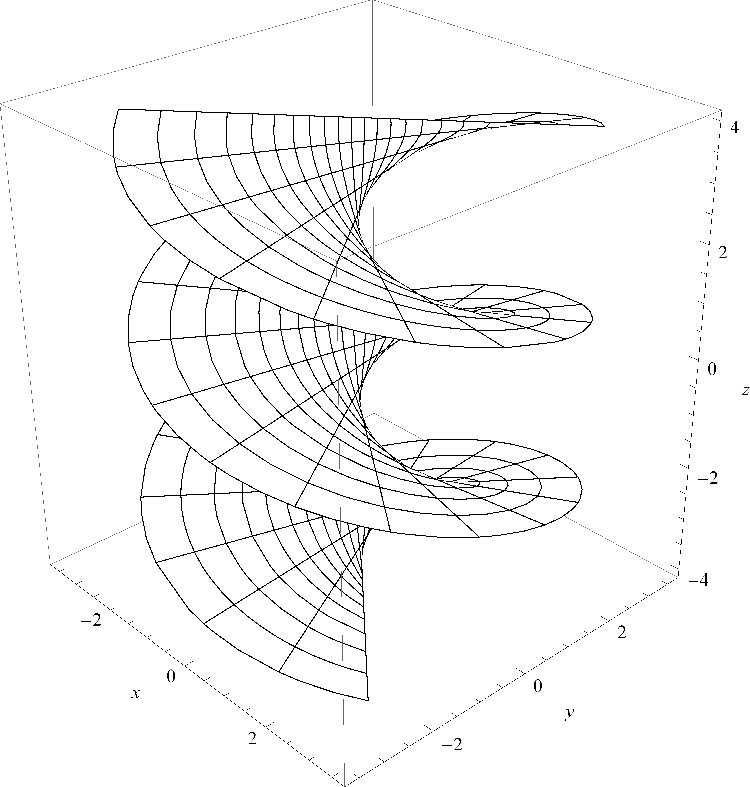
\includegraphics[width=0.5\textwidth]{figures/helicoid.pdf}
      \caption{Helicoid.}
      \label{fig:helicoid}
    \end{figure}
  \end{ex}

  \newcommand{\zint}[2]{\Re#1\int\!#2\,dz}
  % TODO: Catenoid.
  \begin{ex}
    \label{ex:catenoid}
    Let $f = -\frac{e^{-z}}{2}$ and $g = -e^z$, then by the first Weierstrass-Enneper representation, we have
    \begin{multicols}{2}
      \begin{align*}
        x^1 &= \zint{}{-\frac{e^{-z}}{2}\left(1 - e^{2z}\right)}\\
        &= \zint{}{\frac{-e^{-z} + e^z}{2}}\\
        &= \zint{}{\sinh z}\\
        &= \Re\cosh z\\
        &= \cosh u \cos v
      \end{align*}\break
      \begin{align*}
        x^2 &= \zint{}{i\cdot-\frac{e^{-z}}{2}\left(1 + e^{2z}\right)}\\
        &= -\zint{i}{\frac{e^{-z} + e^z}{2}}\\
        &= -\zint{i}{\cosh z}\\
        &= -\Re i\sinh z\\
        &= \Im \sinh z\\
        &= \cosh u \sin v
      \end{align*}
    \end{multicols}
    \begin{align*}
      x^3 &= \zint{2}{-\frac{e^{-z}}{2}\cdot -e^{2z}}\\
      &= \zint{2}{\frac{1}{2}}\\
      &= \Re z\\
      &= u.
    \end{align*}

    This gives us $\bx(u, v) = (\cosh u \cos v, \cosh u \sin v, u)$, which is a catenoid as illustrated in Figure~\ref{fig:catenoid}.
    \begin{figure} % fig: Catenoid
      \centering
      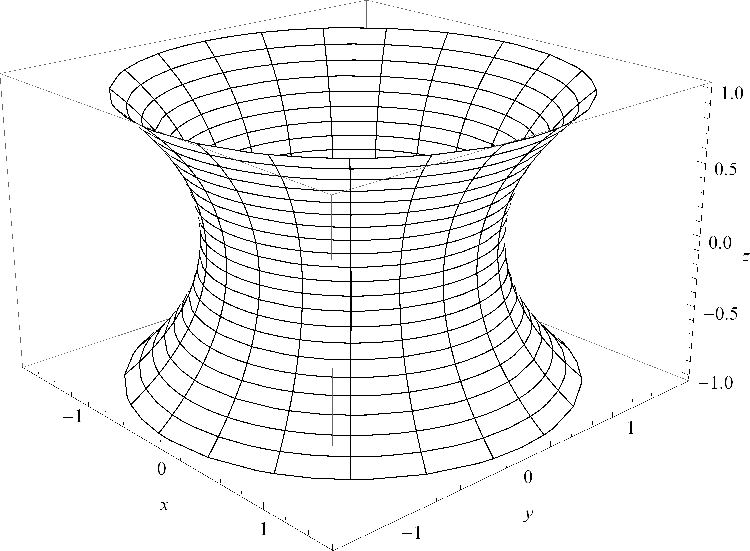
\includegraphics[width=0.5\textwidth]{figures/catenoid.pdf}
      \caption{Catenoid.}
      \label{fig:catenoid}
    \end{figure}
  \end{ex}

  % TODO: Another example.
  \begin{ex}
    Given $F(\tau) = 1$, the surface generated is Enneper's surface, as in Example~\ref{ex:ennepers_surface}. Given that $\tau^3 = \left(f^3 - 3uv^2\right) + i\left(3u^2v - v^3\right)$, observe
    \begin{multicols}{2}
      \begin{align*}
        x^1 &= \tauint{}{(1 - \tau^2)}\\
        &= \tauint{}{1} - \tauint{}{\tau^2}\\
        &= \Re \tau - \frac{1}{3}\Re\tau^3\\
        &= u - \frac{u^3}{3} + uv^2
      \end{align*}\break
      \begin{align*}
        x^2 &= \tauint{}{i(1 + \tau^2)}\\
        &= \tauint{i}{1} + \tauint{i}{\tau^2}\\
        &= \Re i\tau + \frac{1}{3}\Re i\tau^3\\
        &= -\Im\tau - \frac{1}{3}\Im \tau^3\\
        &= - v + \frac{v^3}{3} - vu^2
      \end{align*}
    \end{multicols}
    
    \begin{align*}
      x^3 &= \tauint{2}{\tau}\\
      &= \Re \tau^2\\
      &= (u^2 - v^2).
    \end{align*}
    And we obtain (though with the second coordinate function negated), the standard parameterization of Enneper's surface.
  \end{ex}
